\documentclass[fontsize=12pt]{article}

% TODO: add stats <27-07-22, Markus A> %
% TODO: add misc info about me <27-07-22, Markus A> %

\usepackage{csvsimple}
\usepackage{hyperref}
\usepackage{tabularx}
\usepackage[a4paper]{geometry}
\usepackage{graphicx}

\hypersetup{
    colorlinks=true,
    linkcolor=blue,
    filecolor=magenta,      
    urlcolor=blue,
    pdftitle={Markus Amano CV}
    }

\geometry{
  left=15mm,
  right=15mm,
  top=15mm,
  bottom=15mm,
}

\begin{document}

\begin{center}
  \begin{tabularx}{\textwidth} { 
      >{\raggedright\arraybackslash}X 
    >{\raggedleft\arraybackslash}X  }
    \huge Markus A.G. Amano & CV\\
    \hline
    Website: \url{https://markuspad.com/}& 
    GitHub: \href{https://github.com/inokawazu}{inokawazu}\\
    Email: markus.a.amano[at]gmail.com & \href{https://inspirehep.net/authors/1778034}{iNSPIREHEP}\\
    Nationality: USA & \\
    &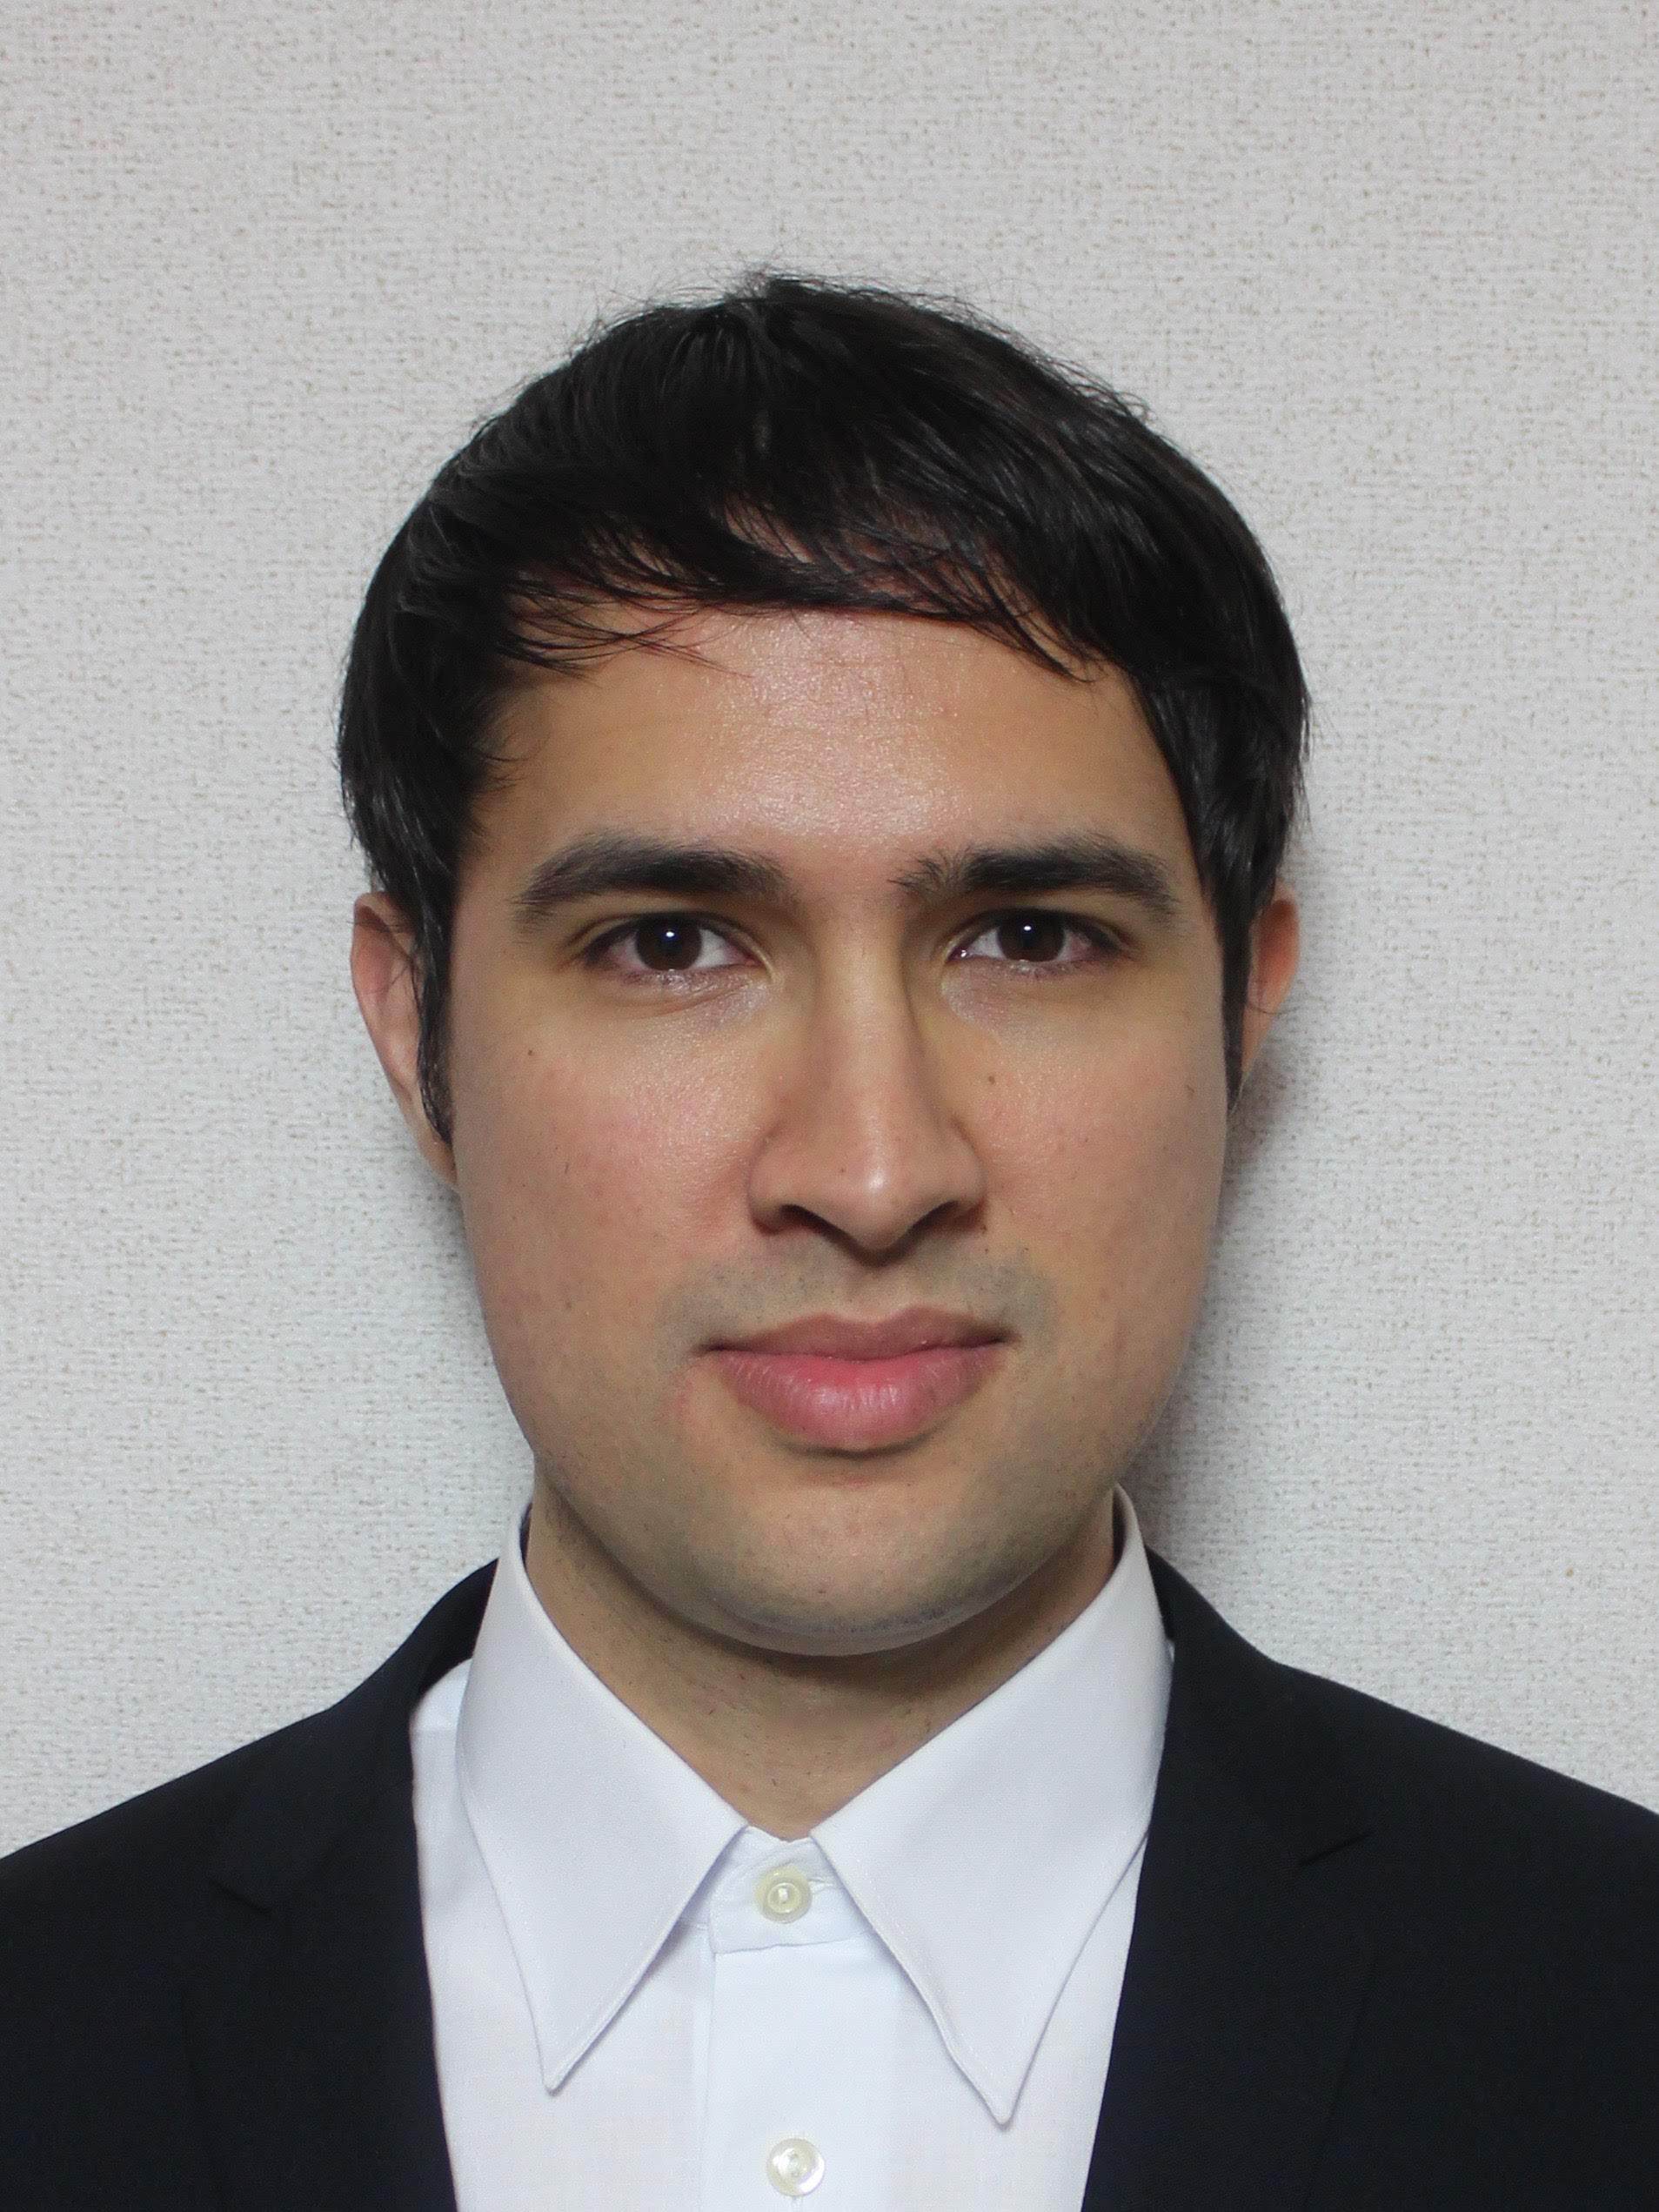
\includegraphics[width=3cm]{data/picture.jpg}\\
  \end{tabularx}
\end{center}


\csvnames{publications}{title=\title,year=\year,arxiv=\arxiv,doi=\doi,journal=\journal}
\csvnames{educations}{degree = \degree,specialization = \specialization,gradyear = \gradyear,entryyear = \entryyear,school = \school,country = \country,city = \city}
\csvnames{appointments}{position=\position,start_year=\startyear,end_year=\endyear,institution=\institution}
\csvnames{recommenders}{name=\name,organization=\organization,position=\position,email=\email, relationship=\relation}
\csvnames{talks}{type=\type,year=\year,month=\month,place=\place}
\csvnames{awards}{award=\award,place=\place,year=\year}
\csvnames{memberships}{organization=\org,start year=\start,end year=\fin,position=\role}


\section*{Publications (Including Preprints)}

% degree,specialization,gradyear,entryyear,school,country,city
\csvreader[publications]{data/publications.csv}{}{
  \textit{\year}\ -\ \textbf{\title}\\
  \ifcsvstrcmp{\doi}{TBD}{}{\href{https://doi.org/\doi}{\doi}\ -\ }
  \ifcsvstrcmp{\arxiv}{TBD}{}{arXiv:\href{https://arxiv.org/abs/\arxiv}{\arxiv}}
  \\
}

\section*{Education}

\csvreader[educations]{data/education.csv}{}{
  \textbf{\degree\ in\ \specialization}\ \entryyear-\gradyear, \school\ -\ \country, \city\\
}

\section*{Appointments/Employments}

\csvreader[appointments]{data/appointments.csv}{}{
  \textbf{\position}\ \ \startyear\ -\ \endyear\\
  \institution
  \\
}

\section*{Miscellaneous}

\subsection*{Given Talks}

\begin{center}
  \begin{tabularx}{\textwidth} { 
      >{\raggedright\arraybackslash}X 
    >{\raggedright\arraybackslash}X  }

    \csvreader[talks]{data/talks.csv}{}{
    \textbf{\type} & \month,\ \year\\
    \textit{\place} & \\
    }
  \end{tabularx}
\end{center}

\subsection*{Awards}

\begin{center}
  \begin{tabularx}{\textwidth} { 
      >{\raggedright\arraybackslash}X 
    >{\raggedright\arraybackslash}X  }

    \csvreader[awards]{data/awards.csv}{}{
    \textbf{\award} & \year\\
    \textit{\place} & \\
    }
  \end{tabularx}
\end{center}

\subsection*{Memberships}

\begin{center}
  \begin{tabularx}{\textwidth} { 
      >{\raggedright\arraybackslash}X 
    >{\raggedright\arraybackslash}X  }

    \csvreader[memberships]{data/memberships.csv}{}{
    \textbf{\role} & \start\ -\ \fin\\
    \textit{\org} & \\
    }
  \end{tabularx}
\end{center}

\end{document}
